\documentclass{proc}

\usepackage[margin=1in]{geometry}
\usepackage{graphicx}

\title{Including Graphics}
\author{Ryan Steiger}
\date{}

\begin{document}

\maketitle

\section{Introduction}

Picture books are just \emph{better}!

\subsection{Including Graphics}

This is a banana in a JPG.

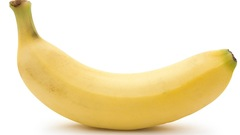
\includegraphics[width=2in]{banana.jpg}

This is a fish, in a chart, in a PNG.

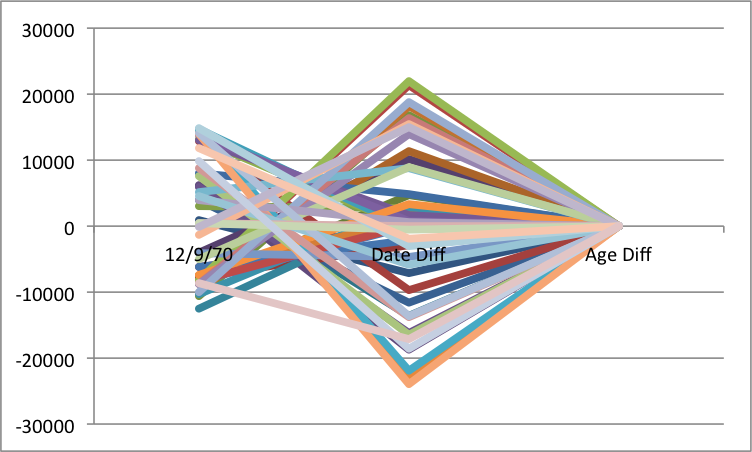
\includegraphics[width=2in]{fish.png}

\subsection{Float: Figure Environment}

In my article, I want to include a JPG image of a banana. You can see this image in Figure~\ref{fig:banana}.

\begin{figure}[htbp]
  \begin{center}
    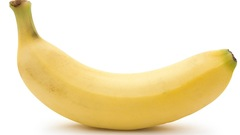
\includegraphics[width=2in]{banana.jpg}
    \caption{This is a banana}
    \label{fig:banana}
  \end{center}
\end{figure}

In my article, I want to include a PNG image of a chart that looks like a fish. You can see this image in Figure~\ref{fig:fish}.

\begin{figure}[htbp]
  \begin{center}
    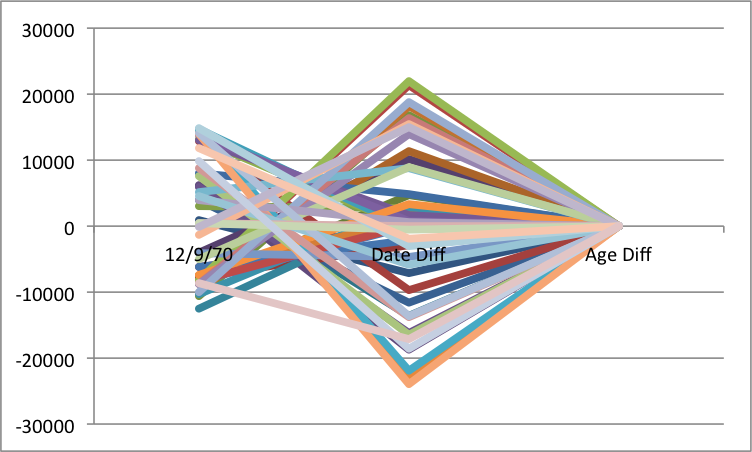
\includegraphics[width=2in]{fish.png}
    \caption{This is a chart that looks like a fish.}
    \label{fig:fish}
  \end{center}
\end{figure}

\section{Conclusion}

Adding images to an article.

\end{document}